% Appendix 8: The Rigid System of Perceptual Perspective
% Source pages: 274–281

\chapter{The Rigid System of Perceptual Perspective}

\srcpage{274}

To construct the rigid system of perceptual perspective, one must solve the problem of
depicting an individual point of picture-space on the picture plane, and obtain a
\emph{unique} solution.  Any point of picture-space must always be depicted by the same
point of the picture plane, regardless of how the corresponding constructions are carried
out.  In addition, one must require that the construction correspond as fully as possible
to natural visual perception.

As proved in Appendix~2, a perfect transmission of the geometry of visual perception on
the picture plane is in principle impossible, which, when applied to depicting an
individual point, means the impossibility of adequately transmitting all three of its
coordinates.  The artist's freedom of choice in the perceptual perspective system
consists, as already mentioned, in deciding which one of the three coordinates to transmit
with distortion, and which ones without.  One must then verify that this choice leads to a
reasonable method of construction on the picture plane.

Since the system to be built should best serve \emph{landscape} painting, in which large
numbers of prominent verticals are absent, we attempt to construct the system by tolerating
distortion in the less significant vertical dimensions.

\srcpage{275}

We formulate the following requirements for the rigid perceptual perspective system under
consideration.  Let the \emph{module} (the unit of linear size) be the depicted length of
a horizontal segment parallel to the picture plane situated on the middle ground at
distance~$l_*$ from the picture plane.  We require that the scales of depiction of
analogous segments on the near and far grounds be consistent with visual perception (relative
to the module), and that the same property hold for all other horizontal segments on all
three grounds; on the far ground we additionally require the same scale consistency for
vertical segments.  Thus, only the vertical dimensions on the middle and near grounds will
be distorted.

To give these general considerations concrete form, we turn to a rigorous formulation of
the problem.

Introduce the linear-perspective and perceptual-perspective coordinate systems with
coordinates $(x_1, y_1)$ and $(x_2, y_2)$ respectively.  A line lying in the subject
plane, perpendicular to the picture plane, and passing through the observer's position,
is naturally taken as the $y_1$-axis (equation $x_1 = 0$); the same position is adopted
for the $y_2$-axis.

If one mentally traces on the subject plane the lines of equal~$l$ and lines perpendicular
to them (forming a coordinate grid), then on the image the lines of equal~$l$ correspond
to horizontal lines, and the perpendicular family corresponds to a series of lines passing
through the principal point of the picture (straight lines in linear perspective, curves in
perceptual perspective).  Each point of the subject plane is thus represented by a unique
point on the image.

To obtain the image of points of picture-space, one must agree on how vertical segments
of picture-space are to be depicted.  Let them also be vertical on the picture plane.
This is a natural requirement, since the picture plane is perpendicular to the subject
plane.  The question of \emph{how large} to make the depiction of a vertical segment turns
out to be more complex.  Along the $y_2$-axis are laid off both images of vertical
segments \emph{and} segments conveying the recession from the picture plane; these must be
reconciled.  Let a vertical object of height~$H$ stand in the picture plane; its top then
projects on the horizon line.  However, the distance from the base of the picture to the
image of the horizon line exceeds this height: in Appendix~3 it turned out to equal
$(1+\pi/4)H$.  Since by hypothesis distortions are to be shifted onto the vertical
dimensions, the object of height~$H$ must be depicted as having size $(1+\pi/4)H$ in
order that its top also falls on the horizon line.

\srcpage{276}

Suppose the top of every object of height~$H$, wherever it stands in picture-space, must
project onto the horizon line.  Then an object of height~$H$ at depth~$l$ must be shown
with image height~$H_2$ satisfying, on the basis of formulas~(1.1) and~(2.6),
\begin{equation*}
  H \int_{0}^{\infty} \frac{P_1(l)}{(1+l)^2}\,dl + H_2
  = H \int_{0}^{l} \frac{P_1(t)}{(1+t)^2}\,dl + H_2 \, .
\end{equation*}
Hence
\begin{equation*}
  H_2 = H\int_{l}^{\infty} \frac{P_1(l)}{(1+l)^2}\,dl.
\end{equation*}
Extending this condition to all other vertical segments, an object of height~$z$ at
depth~$l_B$ is depicted with size
\begin{equation}
  h_2 = z\int_{l_B}^{\infty} \frac{P_1(l)}{(1+l)^2}\,dl.  \tag{8.1}
\end{equation}

We assess the degree of distortion of heights under this method of depiction.  The
visually perceived size of height~$z$ is determined by formulas~(1.3) and~(2.1):
\begin{equation}
  h_2^* = z\,\frac{P_1(l_B)}{1+l_B}.  \tag{8.2}
\end{equation}
Denote by~$\varepsilon$ the ratio of the depicted size of height~$z$ to its visually
perceived size:
\begin{equation}
  \varepsilon = (1+l_B)\displaystyle\int_{l_B}^{\infty}
    \frac{P_1(l)}{(1+l)^2}\,dl \ [P_1(l_B)]^{-1}.  \tag{8.3}
\end{equation}
Using the specific dependence $P_1(l_B) = 1 + \arctan l_B$, the relation between $\varepsilon$
and~$l_B$ can be represented as a graph (Fig.\,8.1), whose general character is unchanged
for other specific forms of~$P_1$.

\begin{figure}[H]
    \centering
    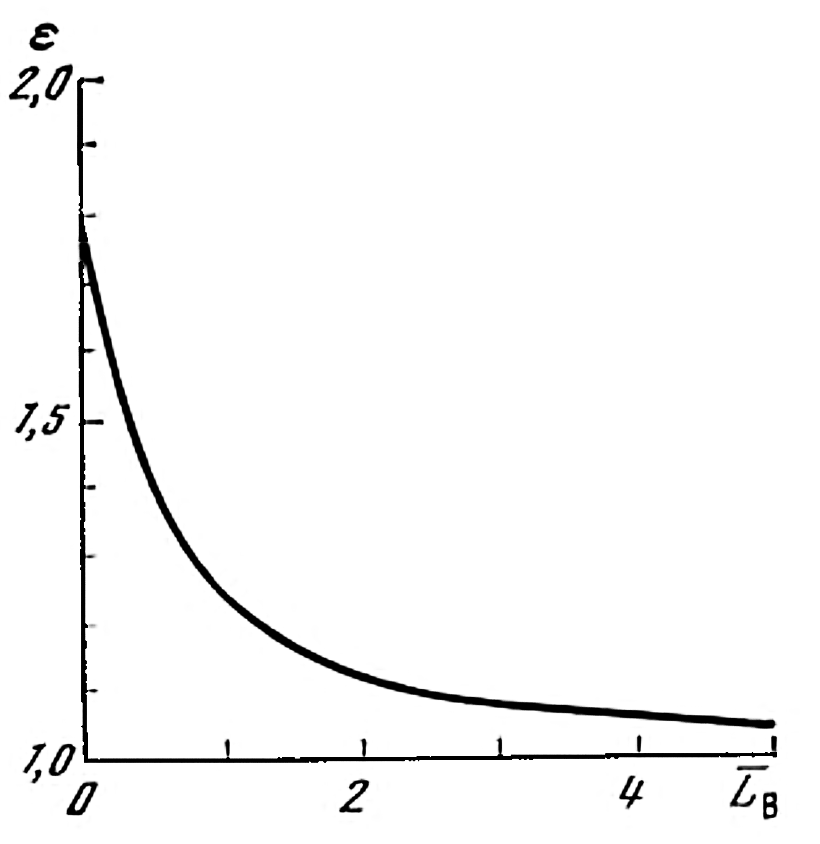
\includegraphics[width=0.4\linewidth]{figures/f8.1.png}
\end{figure}
\figblock{8.1}{Graph of the distortion factor~$\varepsilon$ (ratio of depicted height to
  visually perceived height) as a function of depth~$l_B$.  The distortion is significant
  only for the nearest zone; from $l_B \approx 4$ onward $\varepsilon \approx 1$, and
  exactly $\varepsilon = 1$ as $l_B \to \infty$.}

\srcpage{277}

This graph conveys one extremely important circumstance: the chosen type of distortion,
characterised by~$\varepsilon$ (its deviation from unity), is significant only for the
nearest regions of space.  Beginning from $l_B \approx 1$, the value of~$\varepsilon$
exceeds unity by only about 20\% in the case under consideration, and after $l_B \approx 4$
it may be approximately taken as unity.  The exact value $\varepsilon = 1$ is attained
only as $l_B \to \infty$.  Consequently, if depicting a landscape that has no tall objects
in the foreground, these formally existing distortions cannot manifest themselves.

We now introduce the functions
\begin{align}
  P_2(l) &= \frac{P_1(l)}{1+l},  \tag{def.}\\
  P_3(l) &= \int_0^{l} \frac{P_1(l)}{(1+l)^2}\,dl,  \tag{def.}
\end{align}
so that $P_3(\infty) = \int_0^\infty P_1(t)/(1+t)^2\,dt$.  We give a summary of the
final formulas describing the variant of the rigid perceptual perspective system discussed.

Let $b$, $X$, $z$ be the coordinates of some point in picture-space, where $z$ is the
height above the subject plane and $X$ is the lateral coordinate.  Let the corresponding
quantities in the picture plane be $y_2$, $x_2$, $h_2$.  Then
\begin{equation}
  y_2 = H\,P_3(l),\quad
  x_2 = X\,P_2(l),\quad
  h_2 = z\bigl[P_3(\infty) - P_3(l)\bigr].  \tag{8.4}
\end{equation}

If the module is taken as the image of a horizontal segment parallel to the picture plane,
situated at distance~$l_*$, and for simplicity numerically equal to the eye height~$H$,
the formulas become
\begin{equation}
  \tilde{y}_2 = M\,\frac{P_3(l)}{P_2(l_*)},\quad
  \tilde{x}_2 = \frac{MX\,P_2(l)}{H\,P_2(l_*)},\quad
  \tilde{h}_2 = \frac{M z \ P_3(\infty) - P_3(l)}{H \ P_2(l_*)},  \tag{8.5}
\end{equation}
where $M$ is the dimensional unit magnitude depending on the size of the picture.  If
it is desired to measure $y_2$ from the lower edge of the picture corresponding to
$l = l_k$,
\begin{equation}
  \tilde{y}_2 = M\,\frac{P_3(l) - P_3(l_k)}{P_2(l_*)}.  \tag{8.6}
\end{equation}

The constructed perspective system possesses the important property of
\emph{commutativity}.  This property means that the ``transition'' from some point~$A$
to another point~$B$, decomposed into elementary movements ``away'', ``toward'',
``sideways'', and ``upward'', is independent of the order of these elementary movements.
If one wished to transmit vertical segments also in their visually perceived magnitudes,
the commutativity property would be violated.  Indeed, let one need to pass from
point~$A$ with coordinates $(l = X = z = 0)$ to point~$B$ with
$(l = l_B,\; X = 0,\; z = H_1)$.  Moving first horizontally then vertically,
the distance of the depicted point~$B$ from the picture base is
\[
  HP_3(l_B) + H_1\bigl[P_3(\infty) - P_3(l_B)\bigr];
\]
reversing the order gives the same expression identically.  If, however, the height~$H_1$
is depicted by its visually perceived size
\[
  h^* = H_1\,P_2(l),
\]
then depending on the order of movements the distance turns out to be either
\[
  HP_3(l_B) + H_1P_2(l_B)
\]
or
\[
  H_1 + (H - H_1)P_3(l_B),
\]
which are in general different.\footnote{It is easy to verify that ordinary linear
  perspective possesses the commutativity property.}

\srcpage{278}

Following visual perception thus leads to discontinuities in the image.  Therefore the
``primacy of continuity'' discussed in Chapter~V has a precise mathematical meaning: it
is the fulfilment of the commutativity conditions.

Consider now the case in which the distortions are shifted entirely onto $y_2$, while
$H_2$ and $x_2$ are both to be transmitted without distortion.  Then instead of~(8.4),
\begin{equation}
  x_2 = X\,P_2(l),\quad
  H_2 = z\,P_2(l),\quad
  y_2 = H\bigl[1 - P_2(l)\bigr].  \tag{8.7}
\end{equation}
As was shown above, requiring $H_2$ and $y_2$ to be simultaneously undistorted violates
commutativity.  Thus this variant of the rigid perceptual perspective system does not exist.

This circumstance prompts closer examination of the problem of conveying depth.  All
textbooks on the psychology of visual perception state that the remoteness of a point on
the ground surface may be judged by how close it is to the horizon line in the visual field;
for this reason it was assumed throughout that the depth of a point from the observer is
characterised by the coordinate~$y_2$.  There is, however, an analogous depth indicator---
probably much weaker, but not to be ignored entirely.  Imagine looking along the axis of a
long corridor: the remoteness can be judged not only from the height of a point in the
visual field but also from its horizontal position relative to the walls.  Lowering the
viewpoint to floor level makes this clearest: all $y_2 = 0$, yet the sense of depth does
not vanish.  This permits conveying depth using not only vertical but also horizontal
displacement.  A new coordinate~$\xi$ could be introduced along the $x_2$-axis, measured
from the vertical plane through the principal point.  This situation will not be developed
further here, since such effects are much weaker than the principal effect associated
with~$y_2$, and play a subordinate role in visual perception.

\srcpage{279}

The possibility of shifting the inevitable distortions in various ways allows variants of
perceptual perspective systems to be developed in which these distortions are not
concentrated on one coordinate but distributed among them, in order to seek in this way
optimal systems in some sense.  Such a problem is not considered in the present work.

In conclusion, we clarify the comparative assessments of the two perspective systems given
in the table of Chapter~X.  We give the necessary summary of formulas.

Natural visual perception is described by
\begin{equation}
  x_2^* = X\,P_2(l),\quad y_2^* = H\,P_3(l),\quad h_2^* = z\,P_2(l),  \tag{8.8}
\end{equation}
and the variant of the perceptual perspective system discussed in detail above by
\begin{equation}
  x_2 = x_2^*,\quad y_2 = y_2^*,\quad
  h_2 = z\bigl[P_3(\infty) - P_3(l)\bigr].  \tag{8.9}
\end{equation}
As for the linear perspective system, it is obtained from~(8.8) or~(8.9) by setting
$P_1 \equiv 1$, which gives $P_2(l) = 1/(1+l)$, $P_3(l) = l/(1+l)$, $P_3(\infty) = 1$:
\begin{equation}
  x_1 = \frac{X}{1+l},\quad y_1 = \frac{Hl}{1+l},\quad h_1 = \frac{z}{1+l}.  \tag{8.10}
\end{equation}

In compiling the comparison table, the condition was adopted that the size~$a$ on the
middle ground is the starting module; by definition, this size is therefore transmitted
correctly.  This is marked in both rows of the table by a ``plus'' sign.  Consider the
first row, corresponding to linear perspective.  The size~$b$ on the middle ground is also
transmitted correctly, since a face of a cube parallel to the picture plane is always
depicted as a square in linear perspective; consequently the ratio~$a/b$ is correctly
transmitted on all three grounds.  As follows from~(8.8) and~(8.10), the ratio~$d/d^*$
is correctly transmitted in linear perspective, but the magnitude~$d$ itself is transmitted
with error on all grounds.  Moreover, because linear perspective ignores the constancy
mechanisms described by $P_1(l)$, the quantities $a$, $b$, $d$ on the near and far grounds
are erroneous.  For the same reason the faces not parallel to the picture plane
(parameters $d/a$, $d'/a$, $b'/b$) are incorrectly transmitted on the near and middle
grounds.  Only on the far ground, where $P_1(l)$ becomes practically constant, is there
complete similarity of images in both perspective systems.  As for the perceptual
perspective system (second row), all its errors are connected only with the inadequate
transmission of the magnitude~$h$ on the near and middle grounds.

\srcpage{280}

It is appropriate here to note that linear perspective can be obtained from the rigid
perceptual perspective system by a suitable choice of the allowed distortions.  If one
requires that, in some variant of perceptual perspective, straight lines of objective
space are depicted as straight lines on the picture plane, this imposes on $P_1(l)$ the
condition arising from
\[
  y_1 = a + bx_1 \quad(a,b = \mathrm{const}),\qquad
  b\frac{dx_2}{dy_2} = 1 - \frac{P_1'(l)(1+l)}{P_1(l)} = \mathrm{const},
\]
which, after imposing the additional condition that $P_1(\infty)$ is finite,
gives $P_1(l) = 1$, immediately leading to the linear perspective system.  This result
is interesting in that it allows the linear perspective system to be regarded as a special
case of the perceptual perspective system---not only for distant regions of space but
for the whole of space.

\bigskip
\noindent\textbf{Table of the functions $P_1(l)$, $P_2(l)$, $P_3(l)$.}

\medskip
\begin{center}
\begin{tabular}{r|ccc}
  $l$ & $P_1(l)$ & $P_2(l)$ & $P_3(l)$ \\
  \hline
  $0$     & 1.00 & 1.00 & 0     \\
  $0.5$   & 1.46 & 0.97 & 0.40  \\
  $1.0$   & 1.78 & 0.89 & 0.67  \\
  $1.5$   & 1.98 & 0.79 & 0.86  \\
  $2.0$   & 2.11 & 0.70 & 1.00  \\
  $3.0$   & 2.25 & 0.56 & 1.18  \\
  $5.0$   & 2.37 & 0.39 & 1.37  \\
  $10$    & 2.47 & 0.22 & 1.56  \\
  $\infty$& 2.57 & 0    & 1.78  \\
\end{tabular}
\end{center}

\medskip\noindent
[Here $P_1(l) = 1 + \arctan l$;\; $P_2(l) = P_1(l)/(1+l)$;\;
$P_3(l) = \int_0^l P_1(t)/(1+t)^2\,dt$, evaluated using formula~(3.2).]

In the actual construction of the perceptual perspective system an important role is
played by the choice of the line relative to which all space is conventionally divided into
``left'' and ``right'' parts.  In Ill.\,90 and~100 a vertical through the principal point
of the picture was chosen for this purpose.  The circle of questions connected with this
choice is discussed in the following Appendix.
